% Created 2013-11-18 Mon 20:31
\documentclass[11pt]{article}
\usepackage[utf8]{inputenc}
\usepackage[T1]{fontenc}
\usepackage{fixltx2e}
\usepackage{graphicx}
\usepackage{longtable}
\usepackage{float}
\usepackage{wrapfig}
\usepackage{rotating}
\usepackage[normalem]{ulem}
\usepackage{amsmath}
\usepackage{textcomp}
\usepackage{marvosym}
\usepackage{wasysym}
\usepackage{amssymb}
\usepackage{hyperref}
\tolerance=1000
\author{Jason Walsh}
\date{\today}
\title{Yeoman / Grunt / Bower}
\hypersetup{
  pdfkeywords={javascript, tools, build, chrome, google, gdg},
  pdfsubject={Build Chrome Applications with Bower, Grunt, and Yeoman. Seattle Google Developer Group, November 18, 2013},
  pdfcreator={Emacs 24.3.1 (Org mode 8.2.3c)}}
\begin{document}

\maketitle

\section*{Overview}
\label{sec-1}


\includegraphics[width=.9\linewidth]{gdg_2013-11-18_yo_grunt_bower/toolset.png}

\begin{itemize}
\item Increased visibility in the last year of JavaScript tools
\item Integrate two applications and update the configuration
\item Why do the tools exist
\end{itemize}
\section*{Yeoman, Grunt, and Bower with Packaged Apps and AngularJS}
\label{sec-2}

\begin{quote}
Create a Chrome packaged application that uses the Google Drive API
and an Angular application and add in support for manifest generation. 
\end{quote}
\section*{Setup}
\label{sec-3}

\subsection*{Yeoman}
\label{sec-3-1}

Find the following applications: \emph{generator-chromeapp} and \emph{generator-angular}

\begin{verbatim}
yo
\end{verbatim}

\begin{verbatim}
npm -g install generator-{chromeapp,angular}
\end{verbatim}
\section*{Chrome App Project (gDrive)\hfill{}\textsc{s0}}
\label{sec-4}


\subsection*{Setup}
\label{sec-4-1}

\begin{verbatim}
mkdir -p driveChrome && cd $_
yo chromeapp:app
npm install
\end{verbatim}
\subsection*{Layout}
\label{sec-4-2}

\begin{verbatim}
|-- Gruntfile.js
|-- app
|   |-- bower_components
|   |-- images
|   |-- index.html
|   |-- manifest.json
|   |-- scripts
|   `-- styles
|-- bower.json
`-- package.json
\end{verbatim}
\section*{Chrome App Build}
\label{sec-5}

\subsection*{Building}
\label{sec-5-1}

\begin{verbatim}
grunt
\end{verbatim}

\subsection*{Output}
\label{sec-5-2}

\begin{verbatim}
Running "jshint:all" (jshint) task
>> 2 files lint free.

Running "clean:server" (clean) task

Running "concurrent:test" (concurrent) task
\end{verbatim}
\section*{Chrome App Verify}
\label{sec-6}

\begin{itemize}
\item View the application
\item Tools > Extensions
\item Load Unpacked Extension
\end{itemize}

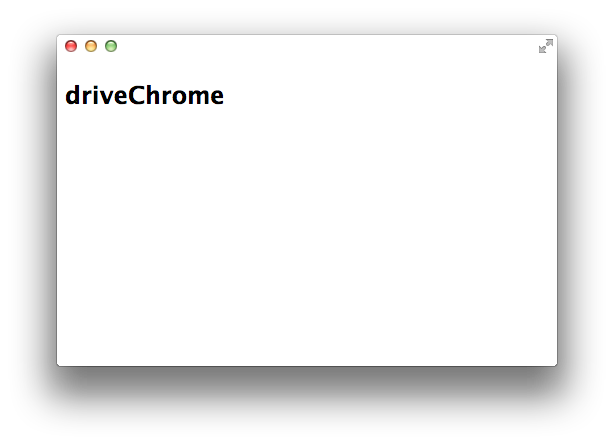
\includegraphics[width=.9\linewidth]{gdg_2013-11-18_yo_grunt_bower/driveChrome.png}
\section*{Chrome App Feature (s3)}
\label{sec-7}

\url{http://developer.chrome.com/apps/angular_framework.html}


\begin{itemize}
\item Update the app functionality
\item driveChrome is a sample application that uses Angular
\item Rebuild as a watcher
\item We're going to remove the hosted dependency on Angular
\end{itemize}
\section*{Chrome App Dependencies (s4)}
\label{sec-8}

\subsection*{Angular}
\label{sec-8-1}

\begin{verbatim}
bower install angular\#1.0.8 --save-dev
\end{verbatim}

\begin{verbatim}
"devDependencies": {
  "angular": "~1.2"
}
\end{verbatim}
\subsection*{Remove Local}
\label{sec-8-2}

\begin{verbatim}
<script src="bower_components/angular/angular.js"></script>
\end{verbatim}
\section*{Chrome App Compression (s5)}
\label{sec-9}

\begin{verbatim}
npm install grunt-contrib-compress --save-dev
\end{verbatim}

\begin{verbatim}
// grunt.loadNpmTasks('grunt-contrib-compress');
    compress: {
      main: {
        options: {
          archive: 'archive.zip'
        },
        files: [
          {src: ['app/**']}
        ]
      }
    },
\end{verbatim}
\section*{Chrome App Linting}
\label{sec-10}

\begin{verbatim}
fixjsstyle Gruntfile.js app
\end{verbatim}

\begin{verbatim}
"indent": 2,
\end{verbatim}

\begin{verbatim}
grunt server
\end{verbatim}
\section*{Angular Project (Buzz) (s10)}
\label{sec-11}


\subsection*{Setup}
\label{sec-11-1}

\begin{verbatim}
mkdir -p buzzAngular && cd $_
yo
npm install
grunt serve
\end{verbatim}
\subsection*{Layout}
\label{sec-11-2}

\begin{verbatim}
|-- Gruntfile.js
|-- app
|   |-- index.html
|   |-- scripts
|   |-- styles
|   `-- views
|-- bower.json
|-- package.json
`-- test
    |-- runner.html
    `-- spec
\end{verbatim}
\section*{Angular Chrome Manifest}
\label{sec-12}


\begin{verbatim}
npm install grunt-chrome-manifest --save-dev
\end{verbatim}

\begin{verbatim}
grunt.loadNpmTasks('grunt-chrome-manifest');
grunt.registerTask('default', ['chromeManifest:dist']);
\end{verbatim}

\begin{verbatim}
chromeManifest: {
  dist: {
    options: {
      buildnumber: 'both',
      background: {
        target: 'scripts/background.js',
        exclude: [
          'background/scripts/chromereload.js'
        ]
      }
    },
    src: 'app',
    dest: 'dist'
  }
}
\end{verbatim}
\section*{Angular Application}
\label{sec-13}

\begin{verbatim}
{
  "name": "Angular Package App Demo",
  "description": "Demo",
  "version": "1",
  "app": {
    "launch": {
      "local_path": "index.html"
    }
  },
  "icons": {
    "16": "icon_16.png",
    "128": "icon_128.png"
  }
}
\end{verbatim}
\section*{Angular Dependencies}
\label{sec-14}

\subsection*{Update dependencies}
\label{sec-14-1}

\begin{verbatim}
"es5-shim": "~2.1.0",
"jquery": "~2.0.3",
"sass-bootstrap": "~3.0.0",
\end{verbatim}
\section*{Yeoman Creates Projects}
\label{sec-15}

\url{http://yeoman.io/}

Other task-oriented build tools: 

\begin{itemize}
\item rails, lein
\end{itemize}

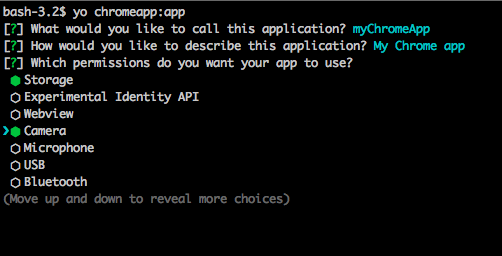
\includegraphics[width=.9\linewidth]{gdg_2013-11-18_yo_grunt_bower/eg-yo.png}
\section*{Yeoman Generators}
\label{sec-16}

\begin{verbatim}
yo --help
\end{verbatim}

\subsection*{Searching}
\label{sec-16-1}

\begin{verbatim}
npm search yeoman-generator chromeapp
npm search yeoman-generator angular
\end{verbatim}
\subsection*{Updating}
\label{sec-16-2}

\begin{verbatim}
npm update -g generator-chromeapp
\end{verbatim}
\section*{Grunt Builds Projects}
\label{sec-17}

\url{http://gruntjs.com/}

\begin{itemize}
\item make, ant, rake, gradle, lein
\end{itemize}

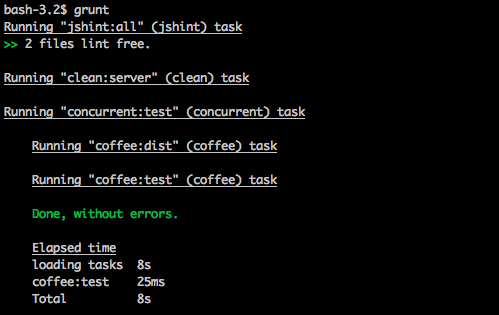
\includegraphics[width=.9\linewidth]{gdg_2013-11-18_yo_grunt_bower/eg-grunt.png}

\begin{verbatim}
grunt --help
\end{verbatim}
\section*{Grunt Plugins}
\label{sec-18}

\begin{itemize}
\item Grunt.js search on GitHub
\item \url{https://npmjs.org/browse/keyword/gruntplugin}
\end{itemize}

Use GitHub for sample plugins: 

\url{https://github.com/search?o=desc&q=Gruntfile.js&ref=cmdform&s=stars&type=Repositories}

\begin{itemize}
\item \url{https://github.com/angular/angular.js/blob/master/Gruntfile.js}
\item \url{https://github.com/eBay/skin/blob/master/Gruntfile.js}
\item \url{https://github.com/fleeting/gruntfile.js/blob/master/gruntfile.js}
\end{itemize}
\section*{Grunt Plugins Angular}
\label{sec-19}

\begin{verbatim}
"grunt-autoprefixer": "~0.4.0",
"grunt-concurrent": "~0.4.1",
"grunt-contrib-coffee": "~0.7.0",
"grunt-contrib-concat": "~0.3.0",
"grunt-contrib-htmlmin": "~0.1.3",
"grunt-contrib-imagemin": "~0.3.0",
"grunt-contrib-jshint": "~0.7.1",
"grunt-contrib-uglify": "~0.2.0",
"grunt-contrib-watch": "~0.5.2",
"grunt-google-cdn": "~0.2.0",
"grunt-ngmin": "~0.0.2",
"grunt-rev": "~0.1.0",
"jshint-stylish": "~0.1.3",
"load-grunt-tasks": "~0.2.0",
"time-grunt": "~0.2.0"
\end{verbatim}

\section*{Grunt plugins Angular DI}
\label{sec-20}

\begin{quote}
You can try to alleviate the pain connected with writing DI
annotations by using build-time tools that would post-process your
code and add annotations automatically. 
\ldots{}
Still, if your build system is Grunt.js based, you can give the
ngmin Grunt.js task (grunt-ngmin)
a try.
\end{quote}

\emph{Mastering Web Application Development with AngularJS} (Kindle Locations 6454-6457).
\section*{Bower Manages Dependencies}
\label{sec-21}

\url{http://bower.io/}

\begin{itemize}
\item ivy, maven, pip
\end{itemize}

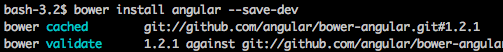
\includegraphics[width=.9\linewidth]{gdg_2013-11-18_yo_grunt_bower/eg-bower.png}

\begin{verbatim}
bower --help
\end{verbatim}
\section*{JavaScript Tools}
\label{sec-22}

\begin{itemize}
\item project templates
\item consistency of style
\item compile on watch
\item static builds
\item HTML rewriting
\item shell script
\item CSS pre-processors
\item dependency checking
\end{itemize}

These all feed into the lifecycle of projects in JavaScript. 
\section*{Friction}
\label{sec-23}

\begin{itemize}
\item Offline access
\item \url{file:////} development locally
\item Version control and sub-module access
\item Server-side integration
\item Old tutorials
\item Local build tools need local NPM hosting
\end{itemize}
\section*{Conclusion}
\label{sec-24}

\begin{itemize}
\item Useful in single page applications
\item Merging generators will likely not result in the correct outcome
\item Still very young
\end{itemize}
\section*{Questions?}
\label{sec-25}

\begin{itemize}
\item Deck: \url{http://bit.ly/I0g5RN}
\item Generator: \url{https://npmjs.org/package/generator-crangular}
\item Examples: \url{https://github.com/jwalsh/gdg_2013-11-18_yo_grunt_bower}

\item Twitter: @jwalsh\_
\item GitHub: jwalsh
\end{itemize}
% Emacs 24.3.1 (Org mode 8.2.3c)
\end{document}